%%%%%%%%%%%%%%%%%%%%%%%%%%%%%%%%%%%%%%%%%%%%%%%%%%%%%%%%%%%%%%%%%%%%%%%%

%%% LaTeX Template for AAMAS-2027 (based on sigconf.tex)
%%% Prepared by the AAMAS-2027 Publication Chairs based on the version from AAMAS-2026. 

%%%%%%%%%%%%%%%%%%%%%%%%%%%%%%%%%%%%%%%%%%%%%%%%%%%%%%%%%%%%%%%%%%%%%%%%

%%% Start your document with the \documentclass command.


%%% == IMPORTANT ==
%%% Use the first variant below to anonymize your submission (no author information shown).
%%% Use the second variant below for the final paper (including author information).
%%% For further information on anonymity and double-blind reviewing, 
%%% please consult the call for paper information
%%% https://warwick.ac.uk/fac/sci/dcs/aamas2027/calls/

%%%% For anonymized submission, use this
\documentclass[sigconf,anonymous]{aamas} 

%%%% For camera-ready, use this
%\documentclass[sigconf]{aamas} 


%%% Load required packages here (note that many are included already).

\usepackage{balance} % for balancing columns on the final page

%%%%%%%%%%%%%%%%%%%%%%%%%%%%%%%%%%%%%%%%%%%%%%%%%%%%%%%%%%%%%%%%%%%%%%%%

%%% AAMAS-2027 copyright block (do not change!)

\makeatletter
\gdef\@copyrightpermission{
  \begin{minipage}{0.2\columnwidth}
   \href{https://creativecommons.org/licenses/by/4.0/}{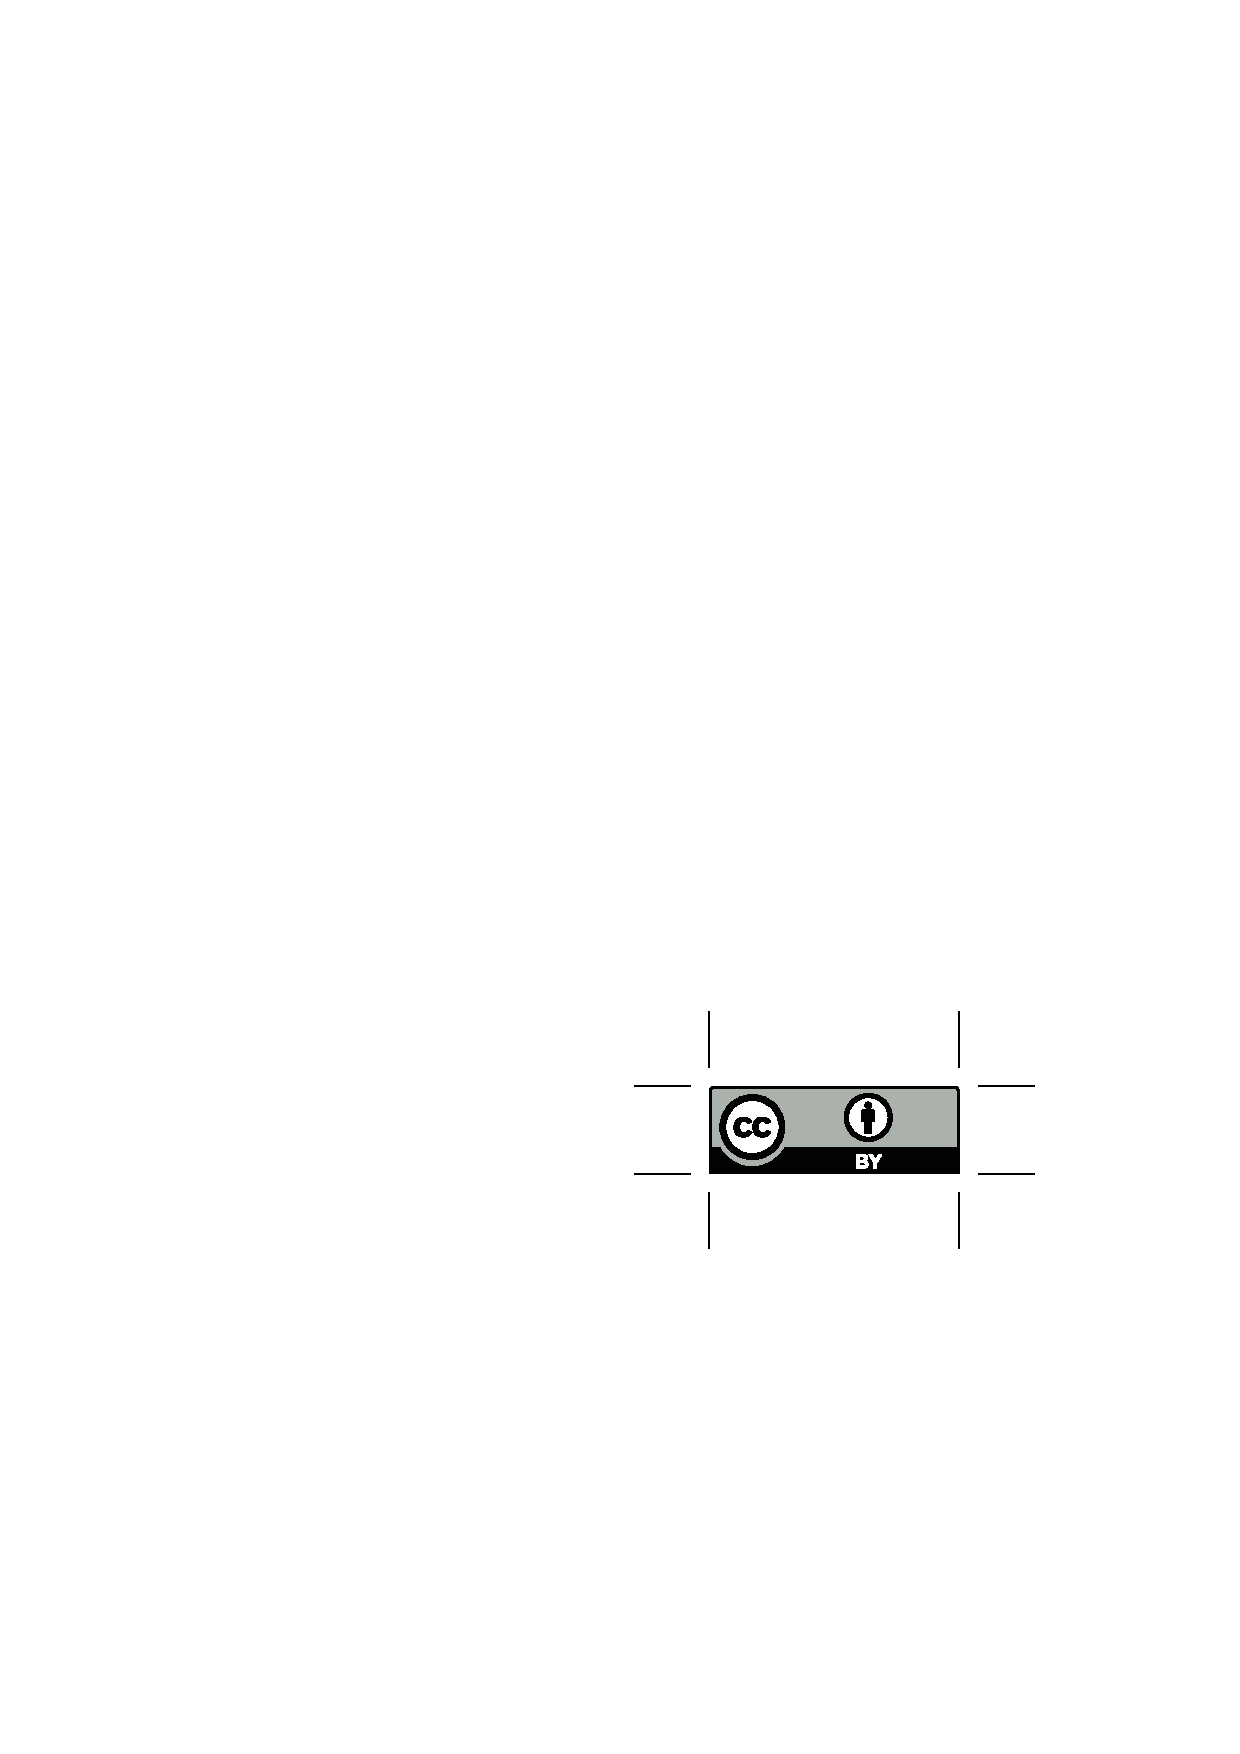
\includegraphics[width=0.90\textwidth]{by}}
  \end{minipage}\hfill
  \begin{minipage}{0.8\columnwidth}
   \href{https://creativecommons.org/licenses/by/4.0/}{This work is licensed under a Creative Commons Attribution International 4.0 License.}
  \end{minipage}
  \vspace{5pt}
}
\makeatother

\setcopyright{ifaamas}
\acmConference[AAMAS 2027]{Proc.\@ of the 26th International Conference
on Autonomous Agents and Multiagent Systems (AAMAS 2027)}{3--7 May 2027}{Hanoi, Vietnam}{M.~Baldoni, F.~Fang, W.~Yeoh, N.~Yorke-Smith (eds.)}
\copyrightyear{2027}
\acmYear{2027}
\acmDOI{}
%\acmPrice{}
\acmISBN{}

%%%%%%%%%%%%%%%%%%%%%%%%%%%%%%%%%%%%%%%%%%%%%%%%%%%%%%%%%%%%%%%%%%%%%%%%

%%% == IMPORTANT ==
%%% Use this command to specify your OpenReview submission number.
%%% In anonymous mode, it will be printed on the first page.

\acmSubmissionID{<<OpenReview submission id>>}

%%% Use this command to specify the track you want to submit your paper to.

\submissionType{Research Paper Track}
%\submissionType{AAAI Track}
%\submissionType{Demonstration Track}
%\submissionType{Blue Sky Ideas Track}
%\submissionType{JAAMAS Track}
%\submissionType{Doctoral Consortium}

%%% Use this command to specify the title of your paper.

\title[AAMAS-2027 Formatting Instructions]{Credit Assignment in Feudal MARL using Goal Counterfactuals}

%%% Provide names, affiliations, and email addresses for all authors.

\author{Arthur Pendragon}
\affiliation{
  \institution{Camelot Castle}
  \city{Camelot}
  \country{United Kingdom}}
\email{king.arthur@camelot.uk}

\author{Nimue}
\affiliation{
  \institution{The Lady's Lake}
  \city{Avalon}
  \country{United Kingdom}}
\email{lady.of.the.lake@avalon.uk}

%%% Use this environment to specify a short abstract for your paper.

\begin{abstract}
Learning to coordinate in long-horizon cooperative tasks is difficult when
agents share a reward that obscures their individual contributions. Feudal
hierarchies structure these tasks through goals assigned by a manager to
workers, but shared feedback does not distinguish useful goal assignments
from progress produced by teammates. We introduce a counterfactual-goal
framework for credit assignment in Feudal multiagent reinforcement learning
with simple spatial waypoint goals. A manager assigns each worker a waypoint
for a fixed horizon, while workers learn control policies using an intrinsic
reward based on reducing their distance to the assigned waypoint. Both levels
are trained with proximal policy optimization. To assign credit to the
manager's decisions, a learned advantage model evaluates alternative
waypoints for one worker while holding the other workers' waypoints fixed.
The resulting counterfactual baseline adjusts the team advantage to provide
a separate learning signal for each worker's goal assignment. This connects
credit assignment across agents and hierarchical levels while retaining an
explicit, interpretable goal definition. We evaluate the approach on a
tightly coupled continuous-control multiagent task involving cooperative
object pushing, where successful manipulation requires coordinated physical
interactions among agents. Our results show that our algorithm can scale to larger agent counts and handle sparse rewards better than the baselines.
% TODO: Replace the placeholder with validated findings for this method.
\textit{[Results pending: specify the comparison methods and principal
empirical finding, including a quantitative result.]}
\end{abstract}


%%% Use this command to specify a few keywords describing your work.
%%% Keywords should be separated by commas.

\keywords{Legends, Myths, Folktales}

%%%%%%%%%%%%%%%%%%%%%%%%%%%%%%%%%%%%%%%%%%%%%%%%%%%%%%%%%%%%%%%%%%%%%%%%

%%% Include any author-defined commands here.
         
\newcommand{\BibTeX}{\rm B\kern-.05em{\sc i\kern-.025em b}\kern-.08em\TeX}

%%%%%%%%%%%%%%%%%%%%%%%%%%%%%%%%%%%%%%%%%%%%%%%%%%%%%%%%%%%%%%%%%%%%%%%%

\begin{document}

%%% The following commands remove the headers in your paper. For final 
%%% papers, these will be inserted during the pagination process.

%\pagestyle{fancy}
%\fancyhead{}

%%% The next command prints the information defined in the preamble.

\maketitle 

%%%%%%%%%%%%%%%%%%%%%%%%%%%%%%%%%%%%%%%%%%%%%%%%%%%%%%%%%%%%%%%%%%%%%%%%

\section{Introduction}

%% The 8 questions
% 1. What is the problem and why do I care?
Teams of autonomous agents have been a key component in problems such as planetary exploration, drone package delivery, warehouse robotics, and  traffic control. Training agent policies for these problems can be done using Multiagent Reinforcement Learning algorithms. 
% 2. Why is it important/difficult?
However, when the problem is a long-horizon, multi-step task, that requires varying degrees of coordination such as object manipulation with multiple agents, current MARL methods struggle to properly assign credit.


% 3. What has been done already in this problem area?
Current approaches apply hierarchical and structural biases to decompose the problem into multiple learners, a manager and a worker. These operate at different timescales and action spaces. This decomposition reduces the action space at the higher levels of the hierarchy leading to more stable learning. 

% 4. What particular problem remains unsolved?
Credit assignment between the higher and lower levels of the hierarchies still remains challenging since current methods rely on domain specific reward definitions for each level, or on experience relabeling which cannot isolate the effects of other agent's goals on each agent's actions. This can lead to suboptimal learning when the environment's reward signal is shared among all levels of the hierarchy.

% 5. How did you solve it?
We introduce a counterfactual-based Feudal MARL framework, that can distill a signal that captures how good a particular agent's goal is, given that other agent's goals stay fixed. We use this signal to train the manager model to produce goals that guide the workers towards effective cooperation policies.

% 6. What is cool about your approach?
 -Idea 1: Our key insight is a goal-aware counterfactual baseline that allows us to capture how an agent's assigned goal will impact the team's performance. The main difference with approaches such as COMA, is that we utilize a counterfactual direction in the manager's latent space to measure how much better a goal change is. Inspired by Feudal Networks, we train our manager by extending the transition policy gradient to a multiagent transition policy gradient that allows our manager to capture the semantics of the team task.

The main difference with approaches such as COMA, is that we utilize a counterfactual direction in the manager's latent space to measure how much better a goal change is. Inspired by Feudal Networks, we train our manager by extending the transition policy gradient to a multiagent transition policy gradient that allows our manager to capture the semantics of the team task.

% - Idea 2: Our key insight is a manager produced intrinsic reward that guides the agents before any extrinsic reward is obtained. The manager produces a vector in latent space for each worker, the workers then get a bonus reward based on how close they got to matching their assigned goal. By decoupling the manager from the agent's state, the agents can execute their policies in a decentralized fashion. The manager optimizes its goals based on how each goal contributed to improving the extrinsic reward.
 


% 7. What were your key results?


% 8. What are the contributions of this paper?

%%%%%%%%%%%%%%%%%%%%%%%%%%%%%%%%%%%%%%%%%%%%%%%%%%%%%%%%%%%%%%%%%%%%%%%%

\section{Background}



%%%%%%%%%%%%%%%%%%%%%%%%%%%%%%%%%%%%%%%%%%%%%%%%%%%%%%%%%%%%%%%%%%%%%%%%

\section{Method}

%%%%%%%%%%%%%%%%%%%%%%%%%%%%%%%%%%%%%%%%%%%%%%%%%%%%%%%%%%%%%%%%%%%%%%%%

\section{Results}


%%%%%%%%%%%%%%%%%%%%%%%%%%%%%%%%%%%%%%%%%%%%%%%%%%%%%%%%%%%%%%%%%%%%%%%%

%%% The acknowledgments section is defined using the "acks" environment
%%% (rather than an unnumbered section). The use of this environment 
%%% ensures the proper identification of the section in the article 
%%% metadata as well as the consistent spelling of the heading.

\begin{acks}
If you wish to include any acknowledgments in your paper (e.g., to 
people or funding agencies), please do so using the `\texttt{acks}' 
environment. Note that the text of your acknowledgments will be omitted
if you compile your document with the `\texttt{anonymous}' option.
\end{acks}

%%%%%%%%%%%%%%%%%%%%%%%%%%%%%%%%%%%%%%%%%%%%%%%%%%%%%%%%%%%%%%%%%%%%%%%%

%%% The next two lines define, first, the bibliography style to be 
%%% applied, and, second, the bibliography file to be used.

\bibliographystyle{ACM-Reference-Format} 
\bibliography{references}

%%%%%%%%%%%%%%%%%%%%%%%%%%%%%%%%%%%%%%%%%%%%%%%%%%%%%%%%%%%%%%%%%%%%%%%%

\end{document}

%%%%%%%%%%%%%%%%%%%%%%%%%%%%%%%%%%%%%%%%%%%%%%%%%%%%%%%%%%%%%%%%%%%%%%%%
